%!TEX root = ../report.tex

\section{Internet Transport Layer}
\subsection{Congestion Control}
One of the transports layers jobs is to handle congestion.
Congestions happens if e.g.\ too many sources send too much data to fast for the network to handle which results in packet loss and long packet delays.\\
Congestion control tries to solve this because without controlling the outgoing traffic, capacity may drop dramatically because of congestion collapse.
\textbf{End-end congestion control} infers congestion only by observing lost packets and delay whereas \textbf{network-assisted congestion control} use informations of routers to detect congestion.
Also an explicit rate can be told to the sender by the network with the second approach.\\

\textbf{Self clocking congestion control} is another approach which sends a new packet for every packet that left the network what the sender knows from ACK messages.
It assumes though that packet loss only occurs due to congestion which is not true for wireless networks for example.

\subsection{Transport Control Protocol (TCP)}
\begin{figure}[h]
  \centering
  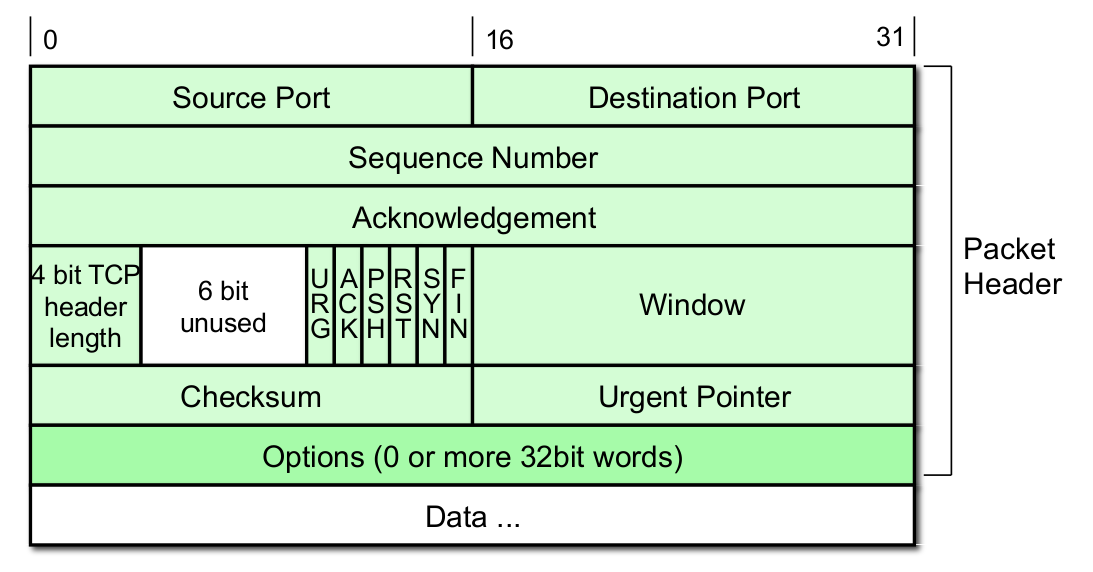
\includegraphics[width=.7\textwidth]{figures/tcp_header.png}
  \caption{TCP Header}\label{fig:tcp_header}
\end{figure}
TCP is an connection oriented protocol that sends packets in order and does retransmission for lost ones.
For the detection of losses, an acknowledgement flag (ACK) is used.
It has an mechanism to avoid losses as good as possible by not overloading the receiver (size of rwin) and network (cwin) that adjusts the sending window to $swin = \min(rwin,cwin)$.\\

A connection is established with the TCP handshake which consists of a SYN, SYNACK and ACK message.
In that, the receiver tells the sender its maximum segment size (MSS) which represents the maximum size of a TCP segment it is able to receive.
When this is done, TCP continues with the so called \textbf{slow start} where the cwin is 1 MSS\@.
To quickly ramp up the transmission, the cwin is increased exponentially until a sender threshold is met.
TCP then enters the congestion avoidance phase where the cwin is increased linearly.
If a packet gets lost (e.g.\ 3 duplicate ACKs), the thrshold is cut in half.
\textbf{With fast recovery}, cwin also cut in half an congestion avoidance starts again.
\textbf{Without fast recovery} cwin is set to 1 MSS again and slow start is applied.
Besides fast recovery, one is also able to use \textbf{fast retransmit}, where not the entire cwin is sent again for missing ACKs but only the missing packet.
Figure~\ref{fig:tcp_sender_congestion_control} shows a good overview over this.\\
\begin{figure}[h]
  \centering
  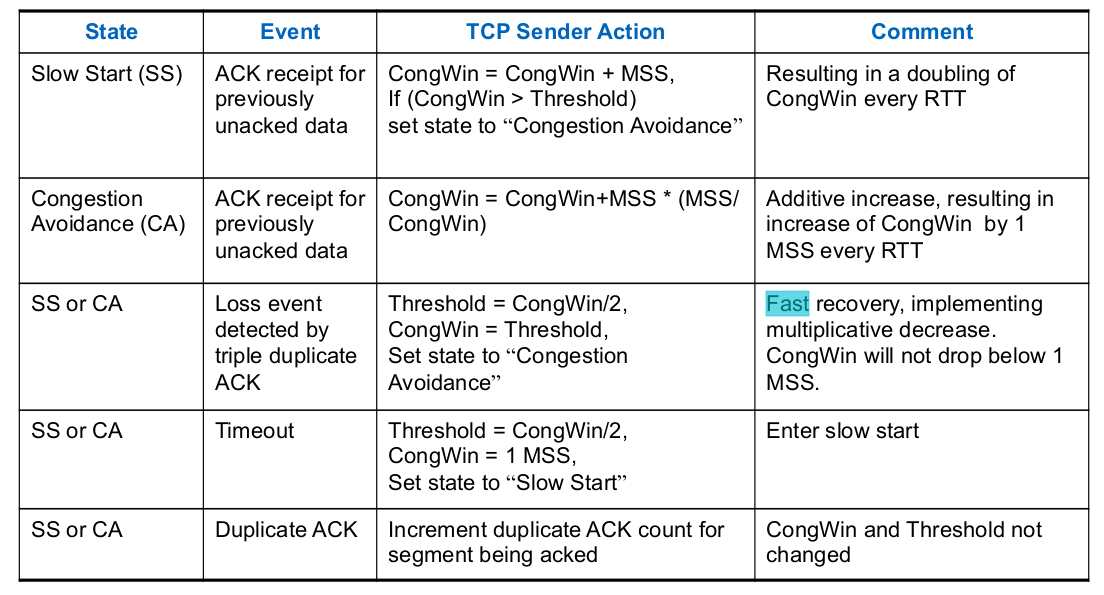
\includegraphics[width=.8\textwidth]{figures/tcp_sender_congestion_control}
  \caption{TCP Sender Congestion Control}\label{fig:tcp_sender_congestion_control}
\end{figure}

\subsubsection*{TCP Fairness}
Two competing TCP sessions will over time get the same bandwidth as indicated in Figure~\ref{fig:tcp_fairness}.
\begin{figure}[h]
  \centering
  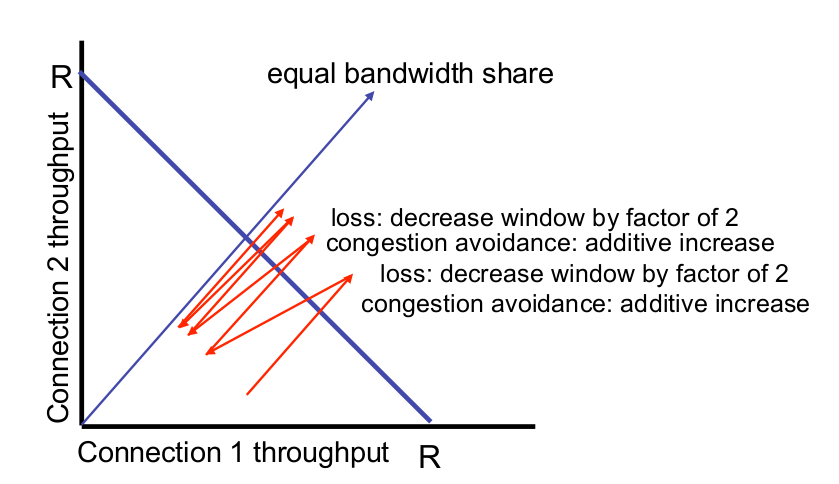
\includegraphics[width=.6\textwidth]{figures/tcp_fairness.png}
  \caption{TCP Fairness}\label{fig:tcp_fairness}
\end{figure}
If an app opens multiple connections though, it might get an higher share of bandwidth because every single connections gets an equal amount independent of the app.
Also multimedia apps often do not want to use TCP, because they do not want the bandwidth to be throttled.
For this reason UDP is oftentimes used with a TCP-friendly rate control.

\subsubsection*{Buffer Bloat}
Large buffers in routes cause problems for TCP connections since once queues are full at the bottleneck, large queueing delays occur.
TCP then gets no early warning about congestion cause no duplicate ACKs are sent but instead sudden timeouts are recognized.
For this reason a large oscillation happens between sending way too much and send way to little (start of slow start again).
Repetition: Rule of thumb for buffers: $\frac{RTT \cdot C}{\sqrt{N}}$ where C is the link bandwidth and N the number of flows.

\subsubsection*{TCP with Explicit Congestion Notification (ECN)}
ECN is a 2 bit field in the IP header.
It can be used on the network layer where endpoints set it to ECT(0) or ECT(1) to declare ECN capable transports and routers set ECN to CE (ECT = ECN capable transport, CE = congestion encountered).\\
On the transport layer, endpoints negotiate ECN at connection setup.
TCP then reacts to CE as if packet is lost with a ECN-Echo to echo back the congestion experienced to the sender which reduces the cwin.
ECT(0) and ECT(1) can be used to differentiate between packets and flows.

\subsubsection*{Data Center TCP (DCTCP)}
DCTCP is an enhancement of TCP's congestion control algorithm that responds to congestion not only regarding its presence but also the amount of congestion.

\subsubsection*{TCP CUBIC}
TCP CUBIC is a loss based congestion control algorithm that optimizes for high bandwidth high latency.
It modifies the window growth algorithm so that the window grows slowly around the maximum size.
Standard TCP outperforms CUBIC in short RTTs though.

\subsubsection*{TCP Vegas}
TCP Vegas is a delay based algorithm that uses $i^{th} RTT > min~RTT + delay~threshold$ to adjust the window size.

\subsubsection*{Delay Gradient TCP}
Delay Gradient TCP uses the delay gradient as a congestion indicator.
It has an average probability of back off independent of RTT and works well in loss-based congestion control flows.

\subsubsection*{TCP Remy}
TCP Remy is an algorithm that tries to find the optimal congestion control protocol for a given network defined by prior network assumptions and goals by using a heuristic search procedure that generates different CC algorithms.

\subsubsection*{TCP BBR (Bottleneck Bandwidth and RTT)}
TCP BBR tries to estimate when the queue will become empty and sends more data just in time.
This is realized by estimating the optimal rate on which the maximum bandwidth and RTT is reached, so the maximum bandwidth-delay product (BDP).
Every ACK measures the RTT and delivery rate by updating the min\_RTT and max\_rate and adapts the rate to assure max\_rate and min\_RTT where the maximum observed bandwidth has priority over $cwin = 2 \cdot min\_RTT \cdot max\_rate$.\\
TCP BBR delivers very good performance and is already deployed in Google WAN backbones.

\subsubsection*{Multipath TCP}
The IETF develops an multipath-aware congestion control transport protocol that can be used for example in smartphones with WLAN and Mobile networks.

